\chapter{Related Work}\label{chap:relatedwork}

Selfish mining is a statistical attack. To analyze profitibality it is therefore beneficial to analytically model selfish mining. In order to study the impact of deviating mining strategies it is very important to represent the blockchain network as close to reality as possible, to estimate realistic results.

Blockchain Mining is most commonly modelled through markov decision processes.
A markovian process is a discrete time stochastic control process. It is generally used to model decision making, where the outcomes are influenced by random processes and the decision of the decision maker.
For the case of selfish mining the selfish miner chooses his next action, so he controls the decision making process. The rest of the network, the block arrival and block propagation can be modelled by stochastic processes. 

Utilizing a markovian model revenue gains can be analytically estimated. \citeauthor{eyal} first described a selfish mining model.
The authors model the network over a set of miners. A miner finds a subsequent block after a time interval that is exponentially distributed. ~\citeauthor{eyal} further define the revenue of a miner as his fraction of total blocks on the longest chain.
The selfish miner withholds mined blocks~\cite{eyal}. This selfish miner now possesses a private chain, which differs from the publicly known chain. Based on the difference between those two chains, the selfish miner performs actions. 
\begin{figure}
\centering
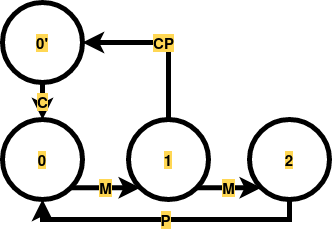
\includegraphics[width=.5\linewidth]{figures/eyal_states.png}
\caption{State Space representation of selfish mining}
\label{fig:eyal_states}
\end{figure}
For clarification the state space and actions are modelled in \ref{fig:eyal_states}. The numbers in the states indicate the lead of the private to the public chain. M denotes mining a block, P publishing the block because of leading by two blocks. CP is an action triggered in state 1 when the miner receives a block. This block will have the same height as the block previously mined by the selfish miner. The selfish miner will compete against this received block by publishing his own. This will cause the selfish miner to transition to 0'. C denotes the transition back to 0. The selfish miner will publish his next mined block immediately or will continue to mine on the next received block in C causing him to transition from 0' to 0.

\citeauthor{eyal} used a Monte Carlo simulation to generate blocks and 1000 Miners operating at identical rates. Block propagation time is considered negligible compared to block generation time~\cite{eyal}. Therefore, communication is considered to be instantaneous. In the case of two branches of identical length, the miners are split up into factions mining on one of the two branches based on the network factor $\gamma$~\cite{eyal}. $\gamma$ resembles a fraction of the network receiving the selfish miner blocks before a simultaneously block sent from another miner.

\citeauthor{optimal_sm} further extended the model to consider all possible actions a selfish miner can perceive. Block propagation time remains unassessed, since it is again considered to be much smaller than block generation time. \citeauthor{optimal_sm} also use the same notion of $\gamma$ like \citeauthor{eyal}. \citeauthor{optimal_sm} model the whole process as a markov decision process.
This markovian model was widely used and adopted in other research directions studying other aspects of selfish mining.

\citeauthor{deepDiveSM} extended the model even further to analyze multiple selfish miners. This resulted in a more complex state space of the markov decision process.

It is not contested by any of the previous research, that network capabilities and communication delay impact selfish mining~\cite{multi_sm}, although most research model block propagation as instantaneous.
Another factor is, that most research which is concerned with selfish mining, builts on top of the model presented by \citeauthor{optimal_sm}
Both factors contribute to the negligence of networking effects, when analyzing selfish mining.

Assuming that the underlying network does influence the system built on top, this master thesis aims to analyze the impact of networking effects on selfish mining.

\citet{xiao_modeling} study the impact on the profitability threshhold and revenue gain of a networking advantage possessed by the selfish miner. They model the network as a graph and find that networking advantage correlates to the betweenness centrality of the selfish miner. Additionally it highly affects the profitability threshhold and revenue gain of the attacker. This indicates that the structure of the network influences the selfish mining strategy. However, this model remains very abstract, since only the peer-to-peer layer and structure is modelled as a graph, disregarding any limitations imposed by physical infrastructure such as bandwidth. Nonetheless, it indicates that the underlying network influences the blockchain overlay, strengthening the assumption that there is a highly influencial dependency between networking effects and selfish mining.

